\section{Gestión del conocimiento}
\subsection{Autoevaluación}
En esta sección se ha cumplido los objetivos correspondientes al 10.
\subsection{Introducción}
\paragraph{}
La gestión del conocimiento busca optimizar el uso de recursos intelectuales y promover la colaboración entre la comunidad. Para ello, se usan herramientas que tienen como objetivo compartir ideas, discutir sobre temas, plantear preguntas y colaborar en la resolución de problemas.
\subsection{Metodología}
\paragraph{}
En Odoo existe una herramienta que ofrece las características que se necesitan para la gestión del conocimiento, para obtenerlo se ha instalado el módulo de Foros. Desde el menú de sitio web en el menú de configuración se puede acceder a los Foros. Si se accede al foro de Ayuda se puede configurar la privacidad, en este caso se ha elegido que solo se accesible por usuarios conectados y también se puede configurar el modo del foro, se ha elegido que se puedan realizar conversaciones en los posts del foro. Además, se ha editado los derechos relacionados con el karma ya que se ha asignado el valor 0 a hacer preguntas y responder preguntas porque no se han verificado los correos. 
\paragraph{}
A continuación, se ha iniciado sesión con un usuario interno, se ha entrado en la página web, se ha navegado al foro y se ha seleccionado el foro de ayuda. Se ha creado una entrada al post con la pregunta correspondiente, cabe destacar que cómo el correo no está verificado el administrador tendrá que entrar al foro y validar la pregunta.
\paragraph{}
Por otro lado, se ha iniciado sesión con 5 usuarios internos diferentes y se han escrito 5 respuestas a la entrada del post. En el foro, con el objetivo de que un usuario, en este caso María, aumente su karma se ha utilizado la cuenta del administrador y se ha votado positivamente la respuesta que ha dado a una pregunta del foro. 
\paragraph{}
Además, se pueden dar insignias a los usuarios, para ello María ha realizado una pregunta en el foro y también ha escrito una respuesta. A continuación, el administrador ha validado la pregunta. El administrador desde la opción de Insignias de la configuración del modulo de Sitio Web, ha hecho clic en otorgar en la insignia de buena pregunta y la insignia de autodidacta, ambas se han asignado a María. 
\paragraph{}
Por otro lado, para probar los privilegios que tiene un usuario con mucho karma, se ha editado la ganancia de karma en el foro para que cuando recibas un voto positivo recibas 100 de karma. Desde la cuenta administrador se ha dado un voto positivo a una respuesta de María, por lo que ahora tiene más de 100 de karma. Además, se ha editado los derechos de karma y se ha asignado 100 de karma para poder editar cualquier mensaje. Por lo que María puede moderar el contenido de otros usuarios. Por último, desde la cuenta del administrador se ha creado la insignia \textit{Gurú} y se la ha otorgado a María. 
\subsection{Resultados y análisis}
\paragraph{}
Se ha conseguido configurar un foro, accesible solo por usuarios conectados y en el que se puedan hacer conversaciones.
Se ha añadido una entrada al foro de Ayuda, con la siguiente pregunta ¿Cuál es el stack tecnológico de la instalación de Odoo?. Además, otros usuarios han respondido a la pregunta con las tecnologías correspondientes. 
\newpage
\begin{figure}[h]
    \centering
    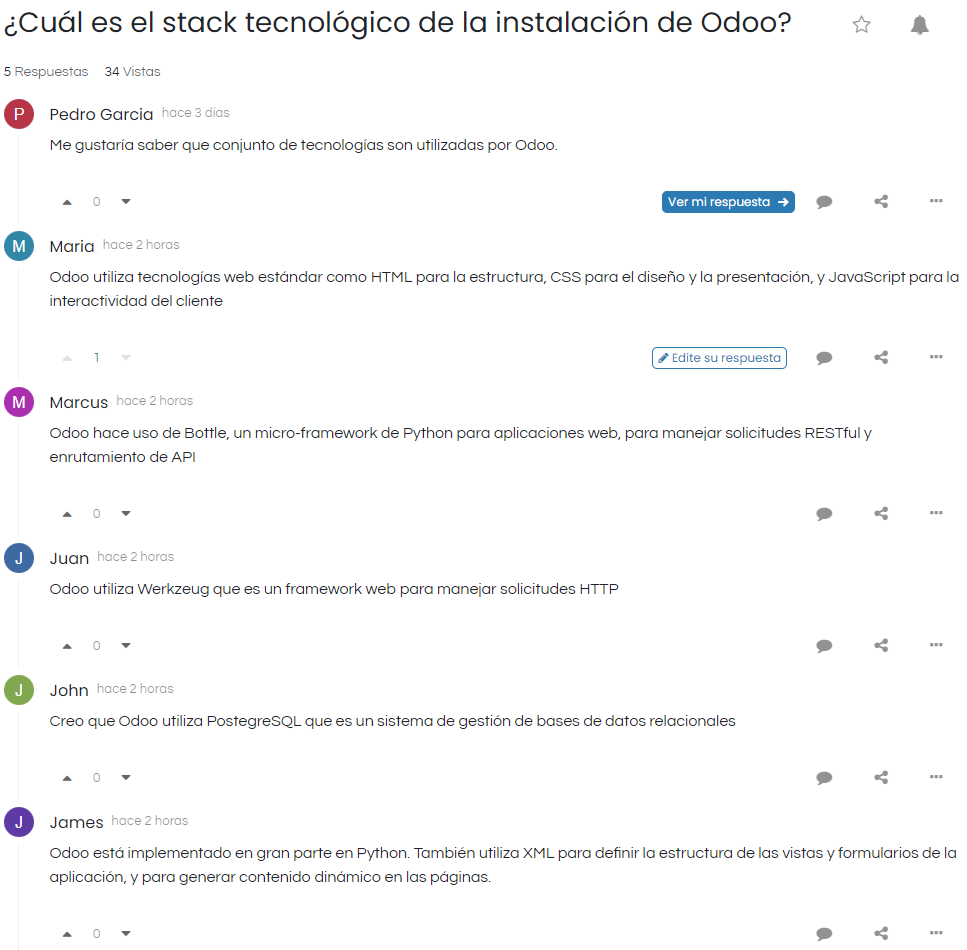
\includegraphics[width=1\linewidth]{fotosGestCon/pregunta1.png}
    \caption{La pregunta ¿Cuál es el stack tecnológico de la instalación de Odoo? en el foro}
    \label{fig:enter-label}
\end{figure}
\paragraph{}
María también ha realizado una pregunta en el foro y ha respondido en esa misma pregunta. Se ha dado un voto positivo a la respuesta de María y se le ha dado la insignia de \textit{Buena pregunta} y \textit{Autodidacta}. 
\newpage
\begin{figure}[h]
    \centering
    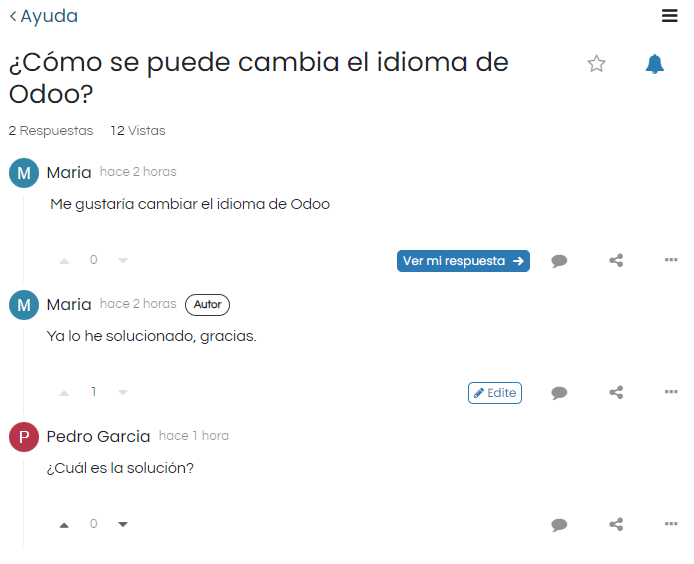
\includegraphics[width=0.75\linewidth]{fotosGestCon/pregunta2.png}
    \caption{Segunda pregunta del foro}
    \label{fig:enter-label}
\end{figure}
\begin{figure}[h]
    \centering
    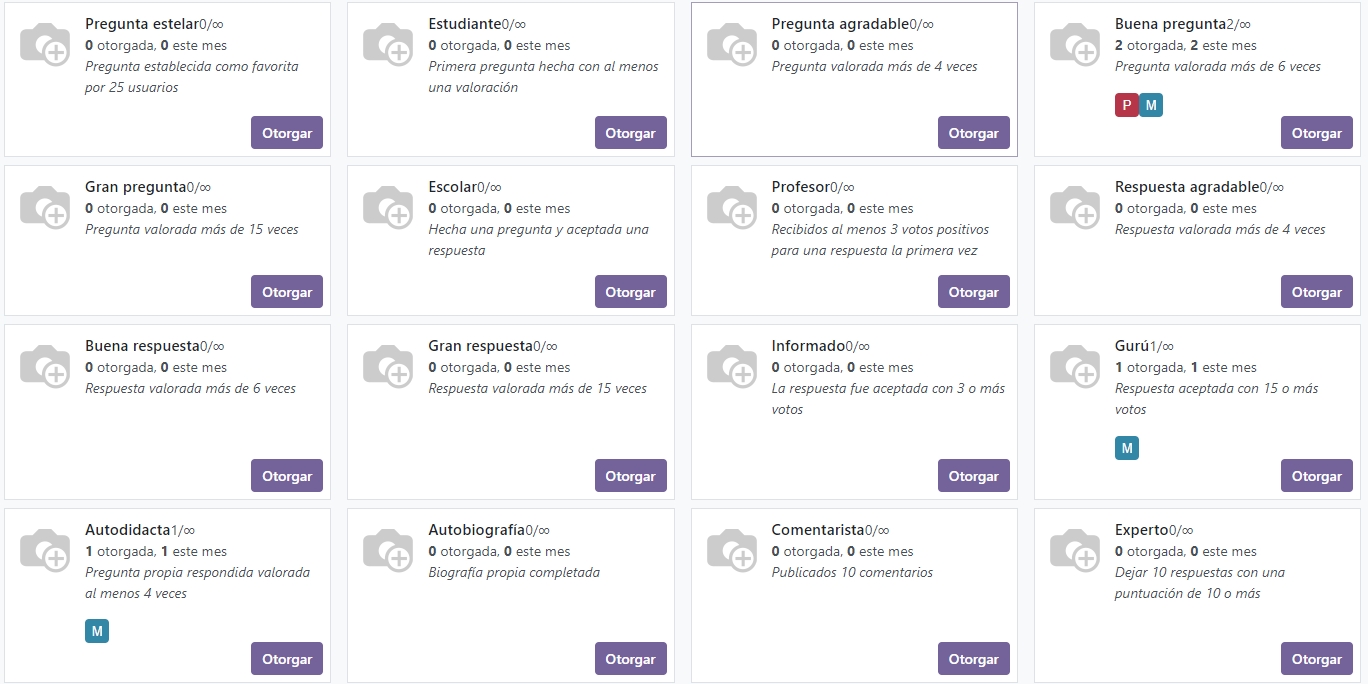
\includegraphics[width=1\linewidth]{fotosGestCon/insignias.png}
    \caption{Lista de insignias y a quién han sido otorgadas}
    \label{fig:enter-label}
\end{figure}
\paragraph{}
Por último, se ha hecho que María alcance unos puntos de karma que le permita moderar el contenido de otros usuarios y además, se le otorgado la insignia de Gurú como se puede ver en la anterior Figura.
\newpage
\begin{figure}[h]
    \centering
    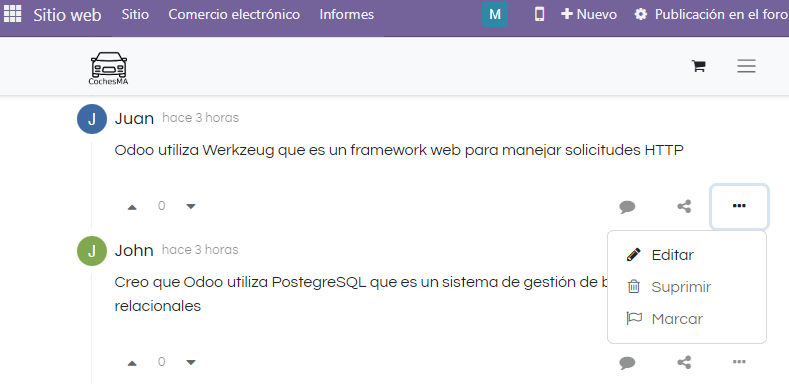
\includegraphics[width=1\linewidth]{fotosGestCon/privilegio.png}
    \caption{Capacidad de editar comentarios de otros usuarios desde la cuenta de María}
    \label{fig:enter-label}
\end{figure}
\subsection{Conclusiones}
\paragraph{}
La implementación de la herramienta de foros en Odoo ha permitido cumplir con los objetivos establecidos. Se han realizado las configuraciones necesarias de manera sencilla, ya que las acciones a realizar han sido intuitivas. 
Este módulo ha demostrado ser una herramienta efectiva para fomentar la gestión del conocimiento y la colaboración de la comunidad para mejorar la página web de la compañía. Sin embargo, deberá haber responsables que moderen el contenido de los foros para asegurar que la información es correcta y adecuada.